\subsection*{Đề thi thử THPTQG 2025 -- 2026 Sở GD\&ĐT ĐỒNG NAI, Lần 2}
\caulc
\Opensolutionfile{ans}[ans/ans-51-26-2-SoGD-DongNai-L2-LC]
\begin{ex}%[2D4N1-1]
	Họ nguyên hàm của hàm số $f(x)=3x^2+2\sin x$ là
	\choice
	{\True $x^3-2\cos x+C$}
	{$x^3+2\cos x+C$}
	{$3x^3+2\cos x+C$}
	{$3x^3-2\cos x+C$}
	\loigiai{
	$\displaystyle\int\limits(3x^2+2\sin x) \mathrm{\,d}x = 3 \cdot \frac{x^3}{3} + 2(-\cos x) + C = x^3 - 2\cos x + C$.
	}
\end{ex}

\begin{ex}%[2H2N2-2]
	Trong không gian $Oxyz$, cho hai điểm $A(2;3;1)$ và $B(-4;-1;5)$. Tọa độ trung điểm $M$ của đoạn thẳng $AB$ là
	\choice
	{$M(6;4;-4)$}
	{$M(-6;-4;4)$}
	{\True  $M(-1;1;3)$}
	{$M(-2;2;6)$}
	\loigiai{
	Tọa độ trung điểm $M$: $x_M = \dfrac{2-4}{2}=-1$; $y_M = \dfrac{3-1}{2}=1$; $z_M = \dfrac{1+5}{2}=3$.\\
	Vậy $M(-1;1;3)$.	
	}
\end{ex}

\begin{ex}%[1D7H1-3]
	Gọi $\Delta$ là tiếp tuyến của đồ thị hàm số $y=x^3+3x$ tại điểm có hoành độ bằng $1$. Hệ số góc của $\Delta$ bằng
	\choice
	{$4$}
	{\True $6$}
	{$1$}
	{$3$}
	\loigiai{
	$y' = 3x^2+3$. Vậy hệ số góc $k = y'(1) = 3\cdot1^2+3 = 6$.
		}
\end{ex}

\begin{ex}%[1D2N3-2]
	Cho cấp số nhân $(u_n)$ có $u_2=6$, $u_3=12$. Công bội của cấp số nhân $(u_n)$ bằng
	\choice
	{$6$}
	{$\dfrac{1}{2}$}
	{\True  $2$}
	{$3$}
	\loigiai{
	Công bội $q = \dfrac{u_3}{u_2} = \dfrac{12}{6} = 2$.
}
\end{ex}

\begin{ex}%[2H5H1-5]
	Trong không gian $Oxyz$, cho mặt cầu $(S)$ có tâm $I(2;-3;-4)$ và tiếp xúc với mặt phẳng $(Oxy)$. Bán kính của mặt cầu $(S)$ bằng
	\choice
	{$3$}
	{$16$}
	{\True $4$}
	{$2$}
	\loigiai{
	$(Oxy)\colon z=0$.\\
	Bán kính mặt cầu $R = d(I, (Oxy)) = |z_I| = |-4| = 4$.
	}
\end{ex}

\begin{ex}%[2D4H2-5]
	Cho hàm số $f(x)$ thỏa mãn $\displaystyle \int\limits_{-2}^{1}f(x)\mathrm{\,d} x=2$. Tính $\displaystyle I = \int\limits_{-2}^1 (1+f(x))\mathrm{\,d} x$.
	\choice
	{$1$}
	{$-1$}
	{$3$}
	{\True $5$}
	\loigiai{
	$\displaystyle I = \int\limits_{-2}^1 1 \mathrm{\,d}x + \int\limits_{-2}^1 f(x) \mathrm{\,d}x = 3 + 2 = 5$.	}
\end{ex}

\begin{ex}%[2D1H2-2]
	Cho hàm số $y=f(x)$ có bảng biến thiên như hình vẽ.
	\begin{center}
		
\begin{tikzpicture}[scale=0.6, font=\footnotesize, line join=round, line cap=round, >=stealth]
			\tkzTab
			[lgt=1.2,espcl=2.5,deltacl=0.8,nocadre=false] 
			{$x$/0.6, $y'$/0.6, $y$/2.5} 
			{$-\infty$, $-1$, $2$, $+\infty$}
			{,+,0,-,0,+,} 
			{-/ $-\infty$, +/ $3$, -/ $-2$ , +/ $+\infty$}
		\end{tikzpicture}
	\end{center}
	Giá trị cực đại của hàm số $f(x)$ là
	\choice
	{\True $3$}
	{$2$}
	{$-2$}
	{$-1$}
	\loigiai{
	Dựa vào bảng biến thiên, ta có $y_{\text{CĐ}}= 3$.
	}
\end{ex}

\begin{ex}%[2H5N2-3]
	Trong không gian $Oxyz$, phương trình chính tắc của đường thẳng đi qua $M(2;1;1)$ và có vectơ chỉ phương $\vec{u}=(2;-1;3)$ là
	\choice
	{$\dfrac{x+2}{2}=\dfrac{y-1}{1}=\dfrac{z+3}{1}$}
	{$\dfrac{x-2}{2}=\dfrac{y+1}{1}=\dfrac{z-3}{1}$}
	{\True $\dfrac{x-2}{2}=\dfrac{y-1}{-1}=\dfrac{z-1}{3}$}
	{$\dfrac{x+2}{2}=\dfrac{y+1}{-1}=\dfrac{z+1}{3}$}
	\loigiai{
	}
\end{ex}

\begin{ex}%[1D1N4-5]
	Hàm số $y=\sin x$ tuần hoàn với chu kỳ
	\choice
	{$T=3\pi$}
	{\True $T=2\pi$}
	{$T=\dfrac{\pi}{2}$}
	{$T=\pi$}
	\loigiai{}
\end{ex}

\begin{ex}%[0D6N4-2]
	Một mẫu số liệu ghép nhóm có tứ phân vị là $Q_1=3$, $Q_2=5$, $Q_3=9$. Khoảng tứ phân vị của mẫu số liệu này là
	\choice
	{$2$}
	{\True $6$}
	{$4$}
	{$5$}
	\loigiai{
	Khoảng tứ phân vị $\Delta_Q = Q_3 - Q_1=9 - 3 = 6$.
	}
\end{ex}

\begin{ex}%[2D5H1-2]
	Cho hai biến cố $A$, $B$ có $\mathrm{P}(B)=0{,}6$ và $\mathrm{P}(A|B)=0{,}5$. Khi đó $\mathrm{P}(AB)$ bằng
	\choice
	{$0{,}5$}
	{\True $0{,}3$}
	{$0{,}8$}
	{$0{,}6$}
	\loigiai{
	Theo công thức xác suất có điều kiện: $P(A|B) = \dfrac{\mathrm{P}(AB)}{\mathrm{P}(B)}$.\\
	Từ đó suy ra công thức nhân xác suất:
	$\mathrm{P}(AB) = \mathrm{P}(B) \cdot \mathrm{P}(A|B)=0{,}6 \cdot 0{,}5 = 0{,}3$.	
	}
\end{ex}

\begin{ex}%[1D6N4-2]
	Nghiệm của phương trình $\log_{2}(x-1)=3$ là
	\choice
	{$x=8$}
	{$x=7$}
	{$x=5$}
	{\True $x=9$}
	\loigiai{
	Điều kiện xác định: $x - 1 > 0 \Leftrightarrow x > 1$.\\
	Ta có:
	$$\log_{2}(x-1) = 3 \Leftrightarrow x - 1 = 2^3\Leftrightarrow x - 1 = 8 \Leftrightarrow x = 9.$$
		}
\end{ex}
\Closesolutionfile{ans}

\cauds
\Opensolutionfile{ans}[ans/ans-51-26-2-SoGD-DongNai-L2-DS]
\begin{ex}%[2D1H4-3]
	Cho hàm số $y=x-3+\dfrac{1}{x-1}$ có đồ thị là $(C)$.
	\choiceTF
	{\True Tập xác định của hàm số là $\mathscr{D}=\mathbb{R}\backslash\{1\}$}
	{\True Tiệm cận xiên của $(C)$ là đường thẳng $y=x-3$}
	{\True Điểm $I(1;-2)$ là tâm đối xứng của $(C)$}
	{Gọi $A, B$ là hai điểm cực trị của $(C)$. Khi đó, ba điểm $A, B$ và $M(3;-2)$ thẳng hàng}
	\loigiai{
		a) Điều kiện $x-1 \ne 0 \Leftrightarrow x \ne 1$.\\
		b) $\lim\limits_{x \to +\infty} (y - (x-3)) = 0$ nên $y=x-3$ là tiệm cận xiên.\\
		c) Đồ thị có TCĐ: $x=1$ và TCX: $y=x-3$.\\
		Giao điểm của hai tiệm cận là $I(1;-2)$.\\
		d) $y' = 1-\dfrac{1}{(x-1)^2}$.\\
		$y'=0 \Leftrightarrow 1-\dfrac{1}{(x-1)^2} = 0 \Leftrightarrow \hoac{&x=0\\&x=2.}$\\
		Với $x = 0 \Rightarrow y = -4 \Rightarrow A(0; -4)$.\\
		Với $x = 2 \Rightarrow y = 0 \Rightarrow B(2; 0)$.\\
	$\vec{AB} = (2;4)$; $\vec{AM} = (3;2)$.\\
	$\vec{AB} \ne k \vec{AM}$ nên $A$, $B$, $M$ không thẳng hàng.
	}
\end{ex}

\begin{ex}%[2D5H2-2]
	Một xét nghiệm chẩn đoán bệnh $X$ có độ nhạy (xác suất người mắc bệnh có kết quả dương tính) là $95\%$ và độ đặc hiệu (xác suất người không mắc bệnh có kết quả âm tính) là $99\%$. Tỉ lệ mắc bệnh $X$ trong cộng đồng là $0{,}5\%$. Chọn ngẫu nhiên một người trong cộng đồng để thực hiện xét nghiệm. Gọi biến cố $A$: "người được xét nghiệm mắc bệnh"; biến cố $B$: "kết quả xét nghiệm dương tính".
	\choiceTF
	{\True $\mathrm{P}(A)=0{,}005$}
	{\True $\mathrm{P}(B|\overline{A})=0{,}01$}
	{$\mathrm{P}(B)=0{,}02$}
	{Nếu xảy ra kết quả dương tính thì xác suất mắc bệnh lớn hơn $0{,}5$}
	\loigiai{
	a) $\mathrm{P}(A)=0{,}005$.
	b) $\mathrm{P}(\overline{B}|\overline{A}) = 0{,}99$. Do đó, $\mathrm{P}(B|\overline{A}) = 1 - \mathrm{P}(\overline{B}|\overline{A}) = 1 - 0{,}99 = 0{,}01$.\\
	c) $\mathrm{P}(B) = (0{,}005 \cdot 0{,}95) + (0{,}995 \cdot 0{,}01) = 0{,}00475 + 0{,}00995 = 0{,}0147$.\\
	d)$\mathrm{P}(A|B) = \dfrac{\mathrm{P}(A \cap B)}{\mathrm{P}(B)} = \dfrac{\mathrm{P}(A) \cdot \mathrm{P}(B|A)}{\mathrm{P}(B)} = \dfrac{0{,}00475}{0{,}0147} \approx 0{,}3231 < 0{,}5$.	
	}
\end{ex}

\begin{ex}%[2H5V3-4]
	Trong không gian $Oxyz$ (đơn vị trên các trục là mét), mặt sân quảng trường trùng với mặt phẳng $(Oxy)$. Một tác phẩm nghệ thuật hình cầu $(S)$ có phương trình $(x+10\sqrt{3})^2+y^2+(z-30)^2=100$. Xét tại thời điểm $14$h, lúc này phương của các tia nắng mặt trời được xác định bởi vectơ $\vec{u}=(1;0;-\sqrt{3})$.
	\choiceTF
	{\True Mặt cầu $(S)$ có tâm $I(-10\sqrt{3};0;30)$ và bán kính $R=10$ (m)}
	{\True Phương trình đường thẳng chứa tia nắng đi qua tâm mặt cầu là $\heva{&x=-10\sqrt{3}+t\\ &y=0\\ &z=30-\sqrt{3}t}$}
	{Gọi $K$ là hình chiếu của tâm $I$ theo phương tia nắng trên mặt sân, khi đó $K(10\sqrt{3};0;0)$}
	{\True Biết rằng hình chiếu của mặt cầu lên mặt sân là một elip, tiêu cự của elip bằng $\dfrac{20}{\sqrt{3}}$}
	\loigiai{
	a) Mặt cầu $(S)$ có tâm $I(-10\sqrt{3};0;30)$ và bán kính $R=10$ (m).\\
	b) Phương trình đường thẳng chứa tia nắng đi qua tâm mặt cầu là $\heva{&x=-10\sqrt{3}+t\\ &y=0\\ &z=30-\sqrt{3}t}$.\\
	c) $K$ là giao điểm của đường thẳng $\heva{&x=-10\sqrt{3}+t\\ &y=0\\ &z=30-\sqrt{3}t}$ và $(Oxy)\colon z = 0$.\\
	Khi đó $K(0;0;0)$.\\
	d) \begin{center}	
		\tdplotsetmaincoords{75}{105}
		\begin{tikzpicture}[tdplot_main_coords, scale=0.1]
			% 1. Vẽ mặt sân Oxy
			\fill[gray!10] (-60,-35,0) -- (40,-35,0) -- (40,35,0) -- (-60,35,0) -- cycle;
			% Trục tọa độ
			\draw[->, black!60] (0,0,0) -- (35,-4.5,0) node[right]{$x$};
			\draw[->, black!60] (0,0,0) -- (0,30,0) node[above]{$y$};
			\draw[->, black!60] (0,0,0) -- (0,0,45) node[above]{$z$};
			% 2. Vẽ bóng Elip trên mặt sân
			\draw[thick, fill=black!40, opacity=0.7] (0,0,0) ellipse [x radius=11.55, y radius=10];
			% Minh họa trục lớn (2a) và trục nhỏ (2b) rõ ràng
			\draw[blue, very thick] (-11.55,1.6,0) -- (11.55,-1.6,0) node[below] {$2b$};
			\draw[red, very thick] (0,-10,0) -- (0,10,0) node[above right] {$2a$};
			% 3. Vẽ hình cầu (S)
			\coordinate (I) at (-17.32, 0, 20);
			% Vẽ khối cầu 3D
			\node[shading=ball, ball color=blue!40, circle, minimum size=2cm] at (I) {};
			\filldraw (I) circle (0.5) node[left,shift={(0,0.5)}] {$I$};
			% 4. Vẽ các tia nắng theo phương u = (1; 0; -sqrt(3))
			\foreach \y in {0, 12.5} {
				\draw[orange!80!black, thick, ->] (-35+\y*0.5, \y, 45) -- (11.55+\y*0.5, \y, -10);
			}
			% 5. Đường dóng giới hạn để thấy bóng elip
			\draw[orange, dashed] (I) -- (0,0,0); % Tia trung tâm
			\draw[gray, dashed] (-17.32, 0, 20) -- (-17.32, 0, -1); 
			% Ký hiệu góc alpha
			\node at (-10,1,-1.5) {$\alpha$};
			\begin{scope}[canvas is yz plane at x=0]
				\draw[thick, black] (2,0) arc (0:60:3);
			\end{scope}
			% Chú thích vectơ phương u
			\node[orange!80!black, font=\boldmath] at (-10, 28, 40) {$\vec{u} = (1; 0; -\sqrt{3})$};
		\end{tikzpicture}	
	\end{center} 
	Gọi $\alpha$ là góc tạo bởi tia nắng và mặt đất ($(Oxy)$). Khi đó $\sin \alpha = \dfrac{|\vec{u} \cdot \vec{n}|}{|\vec{u}| \cdot |\vec{n}|} = \dfrac{\sqrt{3}}{2} \Rightarrow \alpha = 60^\circ$.\\
	Hình chiếu của hình cầu bán kính $R$ theo phương nghiêng góc $\alpha$ so với phương thẳng đứng lên mặt ngang là một Elip có:\\
	Trục bé $2b = 2R = 20 \Rightarrow b = 10$.\\
	Trục lớn $2a = 2\dfrac{R}{\sin \alpha} = 2\dfrac{R}{\sin \alpha} = 2\dfrac{10}{\sin 60^\circ} = \dfrac{40}{\sqrt{3}} \Rightarrow a =\dfrac{20\sqrt{3}}{3}$.\\
	$c = \sqrt{a^2 - b^2} = \sqrt{\left(\dfrac{20\sqrt{3}}{3}\right)^2 - 10^2} = \dfrac{10\sqrt{3}}{3}$.\\
	Vậy tiêu cự của elip $2c = \dfrac{20}{\sqrt{3}}$.
	}
\end{ex}

\begin{ex}%[2D4V2-6]
	Một hồ thủy lợi được vận hành an toàn khi thể tích nước bên trong nó nằm trong khoảng từ $20\,000 \text{ m}^3$ đến $60\,000 \text{ m}^3$. Sau một cơn mưa, người ta đo được lưu lượng nước (tốc độ thay đổi lượng nước) trong hồ là $Q(t)=1000t^3-8000t^2+12\,000t$ ($t$ tính bằng giờ, $Q(t)$ tính bằng $\text{m}^3/\text{giờ}$). Tại thời điểm bắt đầu quan sát ($t=0$), trong hồ có $50\,000 \text{ m}^3$ nước.
	\choiceTF
	{\True Sau $2$ giờ quan sát, thể tích nước trong hồ là $50\,000 + \displaystyle\int\limits_{0}^{2}Q(t)\mathrm{\,d}\,t \text{ m}^{3}$}
	{Trong khoảng thời gian từ $0$ đến $4$ giờ, thể tích nước trong hồ luôn tăng}
	{\True Trong $6$ giờ đầu quan sát, thể tích nước lớn nhất trong hồ là $\dfrac{170\,000}{3} \text{ m}^{3}$}
	{Trong $6$ giờ đầu quan sát, hồ luôn vận hành an toàn}
	\loigiai{
	a) Thể tích nước trong hồ là $\displaystyle V(t) = V(0) + \int\limits_{0}^{t} Q(x)\mathrm{\,d}x$.\\
	Với $t=2$ và $V(0) = 50\,000$, ta có $\displaystyle V(2) = 50\,000 + \int\limits_{0}^{2} Q(t)\mathrm{\,d}t$.\\
	b) Thể tích nước tăng khi lưu lượng $Q(t) > 0$.\\
	$Q(t) = 0 \Leftrightarrow 1000t^{3}-8000t^{2}+12\,000t = 0 \Leftrightarrow \hoac{&x=0\\&x=2\\&x=6.}$\\
	Bảng xét dấu
	\begin{center}
		
\begin{tikzpicture}
			\tkzTabInit[nocadre=false,lgt=1.2,espcl=2.5,deltacl=0.6]
			{$t$/.7 ,$Q(t)$/.7}
			{$-\infty$ , $0$ , $2$ , $6$, $+\infty$}
			\tkzTabLine{ , - , $0$ , + , $0$ , - , $0$ , + , }
		\end{tikzpicture}
	\end{center}
	\noindent c) Bảng biến thiên
		\begin{center}
		
\begin{tikzpicture}
			\tkzTabInit[nocadre=false,lgt=1.2,espcl=2.5,deltacl=0.6]
			{$t$/.7 ,$Q(t)$/.7,$V(t)$/2}
			{$-\infty$ , $0$ , $2$ , $6$, $+\infty$}
			\tkzTabLine{ , - , $0$ , + , $0$ , - , $0$ , + , }
			\tkzTabVar{+/$+\infty$ , -/{} , +/{}, -/{}, +/$+\infty$}
		\end{tikzpicture}
	\end{center}
	Dựa vào BBT, thể tích nước lớn nhất trong $6$ giờ đầu quan sát là\\
	$\displaystyle V(2) = 50\,000 + \int\limits_{0}^{2} Q(t)\mathrm{\,d}t= 50\,000 + \int\limits_{0}^{2} (1000t^3-8000t^2+12\,000t) \mathrm{\,d}\,t = \dfrac{170\,000}{3} \text{ m}^{3}$.\\
	d) Sai. $V(6) = 14\,000 < 20\,000$ nên hồ \textbf{không} luôn vận hành an toàn.
	}
\end{ex}
\Closesolutionfile{ans}

\caukq
\Opensolutionfile{ans}[ans/ans-51-26-2-SoGD-DongNai-L2-KQ]
\begin{ex}%[1D2V3-8]
	\immini{Một Pikachu khám phá "mê cung kỳ lạ" trong mặt phẳng $Oxy$, xuất phát từ $O$ và bước đi vô hạn bước theo quy luật: 
		\begin{itemize}
			\item Bước đầu tiên dài $8$ đơn vị theo tia $Ox$;
			\item Các bước sau luôn rẽ trái $90^\circ$ so với bước liền trước và dài bằng $\dfrac{3}{4}$ bước liền trước.
		\end{itemize}
		Biết rằng Pikachu sẽ tiến đến điểm $M$, độ dài đoạn thẳng $OM$ bằng bao nhiêu đơn vị?}{
		\begin{tikzpicture}[scale=0.5, font=\footnotesize, line join=round, line cap=round, >=stealth]
			\draw[->](-1,0)--(10,0) node[right] {$x$};
			\draw[->](0,-1)--(0,10) node[right] {$y$};
			\draw [ultra thick, black, ->] (8,0) -- (8,6) -- (2,6) -- (2,2);
			\draw (0,0) node [below left] {$O$};
	\end{tikzpicture}}
	\shortans{$6{,}4$}
	\loigiai{
		\begin{center}
				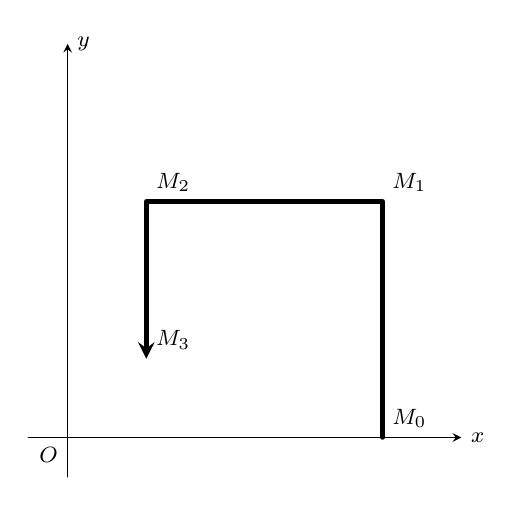
\begin{tikzpicture}[scale=0.5, font=\footnotesize, line join=round, line cap=round, >=stealth]
			\draw[->](-1,0)--(10,0) node[right] {$x$};
			\draw[->](0,-1)--(0,10) node[right] {$y$};
			\draw [ultra thick, black, ->] (8,0) -- (8,6) -- (2,6) -- (2,2);
			\draw (8,0) node[above right]{$M_0$};
			\draw (8,6) node[above right]{$M_1$};
			\draw (2,6) node[above right]{$M_2$};
			\draw (2,2) node[above right]{$M_3$};
			\draw (0,0) node [below left] {$O$};
		\end{tikzpicture}	
		\end{center}
	Gọi $M_n(x_n;y_n)$ là vị trí tọa độ của Pikachu sau $n$ bước di chuyển.\\
	Ta có $x_0$; $x_2$; $x_4$; $\ldots$ là cấp số nhân lùi vô hạn với $u_1 = 8$ và công bội $q=-\left(\dfrac{3}{4}\right)^2=-\dfrac{9}{16}$.\\
	Khi đó 
	$x_M= \dfrac{8}{1-\left(-\dfrac{9}{16}\right)}=\dfrac{128}{25}$.\\
	Tương tự, $y_1$; $y_3$; $y_5$; $\ldots$ là cấp số nhân lùi vô hạn với $u_1 = 6$ và công bội $q=-\left(\dfrac{3}{4}\right)^2=-\dfrac{9}{16}$.\\
	Khi đó 
	$y_M= \dfrac{6}{1-\left(-\dfrac{9}{16}\right)}=\dfrac{96}{25}$.\\
	Suy ra $M\left(\dfrac{128}{25};\dfrac{96}{25}\right)$.\\
	Vậy $OM = \sqrt{\left(\dfrac{128}{25}\right)^2 + \left(\dfrac{96}{25}\right)^2} = 6{,}4$.
	}
\end{ex}

\begin{ex}%[2D5C1-4]
	\immini
	{An chơi trò chơi Minesweeper (gỡ mìn), một trò chơi logic cổ điển, mục tiêu là mở toàn bộ các ô không chứa mìn trên một ``bãi mìn'' có $27$ quả mìn ẩn dưới $27$ ô vuông trong bảng $9\times 9$ ô vuông như hình bên. Nếu mở ô chứa mìn thì An thua cuộc, nếu mở ô không chứa mìn thì trong ô này sẽ hiện số tự nhiên $n$ với $1\le n\le 8$ nhằm cảnh báo cho An rằng, trong số $8$ ô kề quanh ô này có $n$ ô chứa mìn. Hai ô đầu tiên An mở là ô ngay phía trên và ô ngay phía dưới ô trung tâm, hai số ``cảnh báo'' mà hai ô này đưa ra lần lượt là $4$ và $1$.
			
			Nếu ô tiếp theo An mở là ô trung tâm thì xác suất An thua cuộc ngay sau khi mở ô trung tâm là bao nhiêu (không làm tròn các kết quả trung gian, chỉ làm tròn kết quả cuối cùng đến hàng phần trăm)?
			
			\textit{Chú ý: Hai ô vuông đơn vị được gọi là kề nhau nếu chúng chung cạnh hoặc chung đỉnh.}
	}{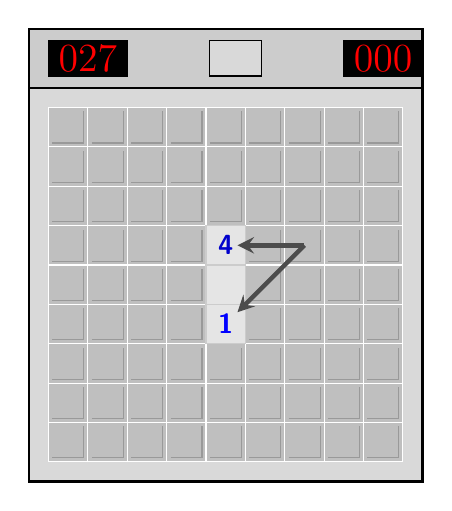
\begin{tikzpicture}[scale=0.5, font=\sffamily\bfseries]
			% 1. Vẽ khung ngoài của bàn cờ
			\draw[fill=gray!30, thick] (-0.5,-0.5) rectangle (9.5, 9.5);
			% 2. Vẽ lưới 9x9 ô vuông
			\foreach \x in {0,1,...,8} {
				\foreach \y in {0,1,...,8} {
					% Vẽ các ô mặc định (màu xám đậm hơn chút để tạo khối)
					\draw[fill=gray!50, draw=white, thin] (\x, \y) rectangle ++(1,1);
					% Hiệu ứng đổ bóng nhẹ cho ô chưa mở
					\draw[gray!80, thin] (\x+0.1, \y+0.1) -- (\x+0.9, \y+0.1) -- (\x+0.9, \y+0.9);
				}
			}
	
			% Ô số 4
			\draw[fill=gray!20, draw=gray!40] (4,5) rectangle ++(1,1);
			\node[blue!80!black] at (4.5, 5.5) {4};
			
			% Ô trung tâm (đang chờ mở)
			\draw[fill=gray!20, draw=gray!40] (4,4) rectangle ++(1,1);
			
			% Ô số 1
			\draw[fill=gray!20, draw=gray!40] (4,3) rectangle ++(1,1);
			\node[blue] at (4.5, 3.5) {1};
			
			% 4. Vẽ các mũi tên chỉ dẫn (giống trong ảnh)
			\draw[ultra thick, -stealth, black!70] (6.5, 5.5) -- (4.8, 5.5); % Mũi tên vào số 4
			\draw[ultra thick, -stealth, black!70] (6.5, 5.5) -- (4.8, 3.8); % Mũi tên vào ô trống
			% 5. Phần bảng điều khiển phía trên (Header)
			\draw[fill=gray!40, thick] (-0.5, 9.5) rectangle (9.5, 11);
			% Ô hiển thị số mìn (027)
			\draw[fill=black] (0, 9.8) rectangle (2, 10.7);
			\node[red, font=\fontfamily{qcr}\selectfont\Large] at (1, 10.25) {027};
			% Ô mặt cười
			\draw[fill=gray!30] (4.1, 9.8) rectangle (5.4, 10.7);
			% Ô hiển thị thời gian (000)
			\draw[fill=black] (7.5, 9.8) rectangle (9.5, 10.7);
			\node[red, font=\fontfamily{qcr}\selectfont\Large] at (8.5, 10.25) {000};			
	\end{tikzpicture}}
	\shortans{$0{,}23$}
	\loigiai{
	\begin{center}
		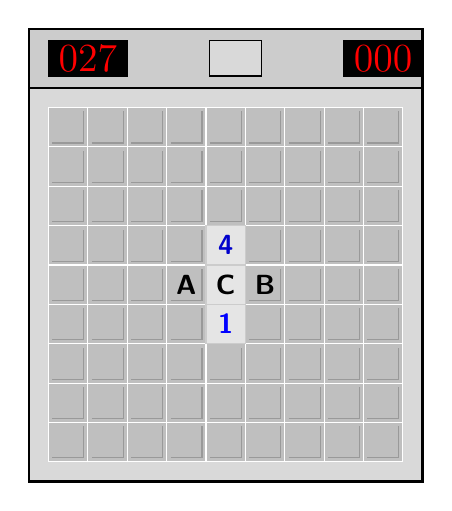
\begin{tikzpicture}[scale=0.5, font=\sffamily\bfseries]
			% 1. Vẽ khung ngoài của bàn cờ
			\draw[fill=gray!30, thick] (-0.5,-0.5) rectangle (9.5, 9.5);
			% 2. Vẽ lưới 9x9 ô vuông
			\foreach \x in {0,1,...,8} {
				\foreach \y in {0,1,...,8} {
					% Vẽ các ô mặc định (màu xám đậm hơn chút để tạo khối)
					\draw[fill=gray!50, draw=white, thin] (\x, \y) rectangle ++(1,1);
					% Hiệu ứng đổ bóng nhẹ cho ô chưa mở
					\draw[gray!80, thin] (\x+0.1, \y+0.1) -- (\x+0.9, \y+0.1) -- (\x+0.9, \y+0.9);
				}
			}
			
			% Ô số 4
			\draw[fill=gray!20, draw=gray!40] (4,5) rectangle ++(1,1);
			\node[blue!80!black] at (4.5, 5.5) {4};
			\node at (3.5,4.5) {A}; \node at (5.5,4.5) {B};
			% Ô trung tâm (đang chờ mở)
			\draw[fill=gray!20, draw=gray!40] (4,4) rectangle ++(1,1);
			\node at (4.5,4.5) {C};
			% Ô số 1
			\draw[fill=gray!20, draw=gray!40] (4,3) rectangle ++(1,1);
			\node[blue] at (4.5, 3.5) {1};
			
			% 5. Phần bảng điều khiển phía trên (Header)
			\draw[fill=gray!40, thick] (-0.5, 9.5) rectangle (9.5, 11);
			% Ô hiển thị số mìn (027)
			\draw[fill=black] (0, 9.8) rectangle (2, 10.7);
			\node[red, font=\fontfamily{qcr}\selectfont\Large] at (1, 10.25) {027};
			% Ô mặt cười
			\draw[fill=gray!30] (4.1, 9.8) rectangle (5.4, 10.7);
			% Ô hiển thị thời gian (000)
			\draw[fill=black] (7.5, 9.8) rectangle (9.5, 10.7);
			\node[red, font=\fontfamily{qcr}\selectfont\Large] at (8.5, 10.25) {000};			
		\end{tikzpicture}
	\end{center}
Gọi $C$ là ô trung tâm. Ta cần tính xác suất
$\mathrm{P}(C \text{ chứa mìn}\mid \text{các dữ kiện đã biết})$.
Hai ô đã mở là:
\begin{itemize}
	\item ô phía trên $C$ cho số $4$;
	\item ô phía dưới $C$ cho số $1$.
\end{itemize}
Kí hiệu:
\begin{itemize}
	\item $A,B,C$ là ba ô chung kề với cả hai ô đã mở (trong đó $C$ là ô trung tâm);
	\item có $5$ ô chỉ kề ô mang số $4$;
	\item có $5$ ô chỉ kề ô mang số $1$.
\end{itemize}
\textbf{Trường hợp 1:} Ô trung tâm $C$ chứa mìn.
Vì ô phía dưới cho số $1$, nên ngoài $C$ ra thì tất cả các ô kề với nó đều không chứa mìn.\\
Khi đó:
\begin{itemize}
	\item trong vùng của ô số $4$ đã có sẵn $1$ quả mìn là $C$;
	\item cần chọn thêm đúng $3$ quả mìn trong $5$ ô còn lại.
\end{itemize}
Số cách là $\mathrm{C}^{3}_{5}=10$.\\
Trong $13$ ô liên quan đang xét có tổng cộng $4$ quả mìn, nên còn $27-4=23$ quả mìn được đặt vào $66$ ô còn lại của bảng.\\
Do đó số trường hợp tương ứng bằng $10\mathrm{C}_{66}^{23}$.\\
\textbf{Trường hợp 2:} Ô trung tâm $C$ không chứa mìn. Khi đó xét hai khả năng sau.\\
\textbf{TH1:} Một trong hai ô $A,B$ chứa mìn.\\
\begin{itemize}
	\item Chọn ô chứa mìn: $\mathrm{C}_2^1=2$ cách;
	\item ô số $4$ cần thêm $3$ quả mìn trong $5$ ô riêng của nó:
	$\mathrm{C}_5^3=10$.
\end{itemize}
Số trường hợp: $2\cdot 10=20$.\\
Trong trường hợp này tổng số mìn ở $13$ ô liên quan là $4$, nên còn $23$ quả mìn đặt vào $66$ ô còn lại.\\
Suy ra số trường hợp: $20\mathrm{C}_{66}^{23}$.\\
\textbf{TH2:} Cả $A,B$ đều không chứa mìn.
\begin{itemize}
	\item ô số $1$ cần đúng $1$ quả mìn trong $5$ ô riêng: $\mathrm{C}_5^1=5$;
	\item ô số $4$ cần đúng $4$ quả mìn trong $5$ ô riêng:
	$\mathrm{C}_5^4=5$.
\end{itemize}
Số trường hợp: $5\cdot5=25$.\\
Lúc này $13$ ô liên quan chứa tổng cộng $5$ quả mìn, nên còn $27-5=22$ quả mìn đặt vào $66$ ô còn lại.\\
Suy ra số trường hợp: $25\mathrm{C}_{66}^{22}$.\\
Vậy xác suất ô trung tâm chứa mìn là
$\mathrm{P}=
\dfrac{10\mathrm{C}_{66}^{23}}
{10\mathrm{C}_{66}^{23}+20\mathrm{C}_{66}^{23}+25\mathrm{C}_{66}^{22}}
\approx 0{,}23$.	
}
\end{ex}

\begin{ex}%[2D4V3-5]
	\immini{Một chiếc cối đá có lòng cối là một paraboloid tròn xoay, với miệng cối là đường tròn có đường kính $40$ cm và chiều sâu lòng cối là $30$ cm. Biết rằng thể tích của lòng cối bằng $a\pi$ ($\text{cm}^3$), giá trị $a$ bằng bao nhiêu?}{
		\begin{tikzpicture}[line join=round, line cap=round, >=stealth, scale=0.8]
			% 2. Vẽ phần thân cối (ngoài)
			% Vẽ một đường bao hơi gồ ghề giả chất liệu đá
			\draw[thick, fill=gray!10] 
			(-2.5, 3.5) -- (2.5, 3.5) % Miệng cối ngoài
			.. controls (2.4, 1) and (1.8, 0) .. (1.5, -0.5) % Cạnh phải
			-- (-1.5, -0.5) % Đáy cối
			.. controls (-1.8, 0) and (-2.4, 1) .. (-2.5, 3.5); % Cạnh trái
			
			% 3. Vẽ lòng cối (Paraboloid mặt cắt)
			% Phương trình: y = 0.75 * x^2
			\draw[ultra thick, fill=white] 
			plot[domain=-2:2, samples=100] (\x, {0.75*\x*\x}) -- cycle;
			
			% 4. Vẽ đế cối (phần gỗ/đá kê bên dưới)
			\draw[thick, fill=gray!30] 
			(-1.8, -0.5) -- (1.8, -0.5) 
			-- (2.2, -1.2) -- (-2.2, -1.2) -- cycle;
			
			% 5. Thêm các vân đá/chấm giả đá (Stippling effect)
			\foreach \i in {1,...,50} {
				\fill[gray] ({rand*2.2}, {0.2 + (3.3-0.2)*rnd}) circle (0.5pt);
			}
			
			% 6. Kí hiệu kích thước (tùy chọn)
			\draw[<->] (-2, 3.8) -- (2, 3.8) node[midway, above] {40 cm};
			\draw[<->] (2.8, 0) -- (2.8, 3) node[midway, right] {30 cm};
			\draw[dashed, gray] (0,0) -- (3,0);
			\draw[dashed, gray] (2,3) -- (3,3);
			
			% 7. Chú thích
			\node at (0, -1.8) {\bf Mặt cắt qua trục};
		\end{tikzpicture}
	}
	\shortans{$6000$}
	\loigiai{
	Lòng cối là vật thể tròn xoay quanh trục $Oy$ tạo bởi Parabol $y=ax^2$.\\
	Điểm $(20;30)$ thuộc đồ thị $\Rightarrow 30 = a \cdot 20^2 \Rightarrow x^2 = \dfrac{40}{3}y$.\\
	$\displaystyle V = \pi \int\limits_0^{30} x^2 \mathrm{\,d}y = \pi \int\limits_0^{30} \frac{40}{3}y \mathrm{\,d}y = 6000\pi$.}
\end{ex}

\begin{ex}%[2D1H3-1]
	Giá trị nhỏ nhất của hàm số $y=x-4\sqrt{x}$ trên đoạn $[0;9]$ bằng bao nhiêu?
	\shortans{$-4$}
	\loigiai{
	Xét trên đoạn $[0;9]$.\\
	$y' = 1 - \dfrac{2}{\sqrt{x}}$.\\
	$y'=0 \Leftrightarrow 1 - \dfrac{2}{\sqrt{x}} = 0 \Leftrightarrow x = 4$.\\
	$y(0) = 0$; $y(4) = -4$; $y(9) = -3$.
	}
\end{ex}

\begin{ex}%[2H2C2-6]
	\immini
	{Một thiết bị hình hộp chữ nhật $ABCD.A'B'C'D'$ có $AB=9$ dm, $AD=12$ dm, $AA'=11$ dm. Bên trong có $2$ vách ngăn song song với mặt đáy $ABCD$ tại độ cao $6$ dm và $9$ dm. Một đường ống gồm $3$ đoạn thẳng nối từ $A$ đến $C'$, đoạn giữa $2$ vách ngăn phải vuông góc với vách ngăn. Độ dài nhỏ nhất của đường ống này là bao nhiêu dm?}{
		\begin{tikzpicture}[scale=0.6,
			line join=round, line cap=round, 
			>=stealth, font=\small,
			% Define 3D parameters for projection
			x={(-0.5cm,-0.4cm)}, % x-axis points "into" the page
			y={(1cm,0cm)},        % y-axis points right
			z={(0cm,1cm)}         % z-axis points up
			]
			
			% --- Define base vertices (front bottom face) ---
			\coordinate (D) at (0,0,0);
			\coordinate (C) at (0,4,0);
			\coordinate (B) at (3,4,0);
			\coordinate (A) at (3,0,0);
			
			% --- Define height ---
			\def\h{4.5}
			\coordinate (A') at ($(A)+(0,0,\h)$);
			\coordinate (B') at ($(B)+(0,0,\h)$);
			\coordinate (C') at ($(C)+(0,0,\h)$);
			\coordinate (D') at ($(D)+(0,0,\h)$);
			
			% --- Define intermediate planes ---
			\def\hI{2}
			\coordinate (AI) at ($(A)+(0,0,\hI)$);
			\coordinate (BI) at ($(B)+(0,0,\hI)$);
			\coordinate (CI) at ($(C)+(0,0,\hI)$);
			\coordinate (DI) at ($(D)+(0,0,\hI)$);
			
			\def\hII{3}
			\coordinate (AII) at ($(A)+(0,0,\hII)$);
			\coordinate (BII) at ($(B)+(0,0,\hII)$);
			\coordinate (CII) at ($(C)+(0,0,\hII)$);
			\coordinate (DII) at ($(D)+(0,0,\hII)$);
			
			\coordinate (M) at (1.2, 1.8, \hI);
			\coordinate (N) at (1.2, 1.8, \hII);
			
			% --- Draw hidden parts (dashed) ---
			\draw[dashed, thin, gray] (A) -- (D) -- (C);
			\draw[dashed, thin, gray] (D) -- (D');
			\draw[dashed, thin, gray] (AI) -- (DI) -- (CI);
			\draw[dashed, thin, gray] (AII) -- (DII) -- (CII);
			
			% --- Draw internal thick path (dashed, prominent) ---
			\draw[dashed, line width=1.8pt, black] (A) -- (M) -- (N) -- (C');
			
			% --- Draw visible parts (solid) ---
			\draw[thick] (A') -- (B') -- (C') -- (D') -- cycle;
			\draw[thick] (B') -- (B) -- (C) -- (C');
			\draw[thick] (A') -- (A) -- (B); % Added missing edge A'-A for full cuboid
			
			% Draw lines of the intermediate planes
			\draw[thin, gray] (AI) -- (BI) -- (CI);
			\draw[thin, gray] (AII) -- (BII) -- (CII);
			
			% --- Vertices and intermediate points points ---
			% Visible vertices (solid dots)
			\fill[black] (A') circle (1.5pt);
			\fill[black] (B') circle (1.5pt);
			\fill[black] (C') circle (1.5pt);
			\fill[black] (D') circle (1.5pt);
			\fill[black] (A) circle (1.5pt);
			\fill[black] (B) circle (1.5pt);
			\fill[black] (C) circle (1.5pt);
			\fill[black] (D) circle (1.5pt);
			
			% Intermediate path points (open circles)
			\draw[thick, fill=white] (M) circle (2.5pt);
			\draw[thick, fill=white] (N) circle (2.5pt);
			
			% --- Labels ---
			\node[above, xshift=2pt] at (A') {$A'$};
			\node[above] at (B') {$B'$};
			\node[above, xshift=-2pt] at (D') {$D'$};
			\node[above] at (C') {$C'$};
			
			\node[below, xshift=-2pt] at (B) {$B$};
			\node[right, yshift=-4pt] at (C) {$C$};
			\node[left, xshift=2pt] at (A) {$A$};
			\node[below, xshift=3pt, yshift=2pt] at (D) {$D$};
			
			\node[above, xshift=3pt] at (N) {$N$};
			\node[below, xshift=3pt] at (M) {$M$};
			
		\end{tikzpicture}
	}
	\shortans{$20$}
	\loigiai{
	\begin{center}
		\begin{tikzpicture}[scale=0.6,
			line join=round, line cap=round, 
			>=stealth, font=\small,
			% Define 3D parameters for projection
			x={(-0.5cm,-0.4cm)}, % x-axis points "into" the page
			y={(1cm,0cm)},        % y-axis points right
			z={(0cm,1cm)}         % z-axis points up
			]
			
			% --- Define base vertices (front bottom face) ---
			\coordinate (D) at (0,0,0);
			\coordinate (C) at (0,4,0);
			\coordinate (B) at (3,4,0);
			\coordinate (A) at (3,0,0);
			
			% --- Define height ---
			\def\h{4.5}
			\coordinate (A') at ($(A)+(0,0,\h)$);
			\coordinate (B') at ($(B)+(0,0,\h)$);
			\coordinate (C') at ($(C)+(0,0,\h)$);
			\coordinate (D') at ($(D)+(0,0,\h)$);
			
			% --- Define intermediate planes ---
			\def\hI{2}
			\coordinate (AI) at ($(A)+(0,0,\hI)$);
			\coordinate (BI) at ($(B)+(0,0,\hI)$);
			\coordinate (CI) at ($(C)+(0,0,\hI)$);
			\coordinate (DI) at ($(D)+(0,0,\hI)$);
			
			\def\hII{3}
			\coordinate (AII) at ($(A)+(0,0,\hII)$);
			\coordinate (BII) at ($(B)+(0,0,\hII)$);
			\coordinate (CII) at ($(C)+(0,0,\hII)$);
			\coordinate (DII) at ($(D)+(0,0,\hII)$);
			
			\coordinate (M) at (1.2, 1.8, \hI);
			\coordinate (N) at (1.2, 1.8, \hII);
			
			% --- Draw hidden parts (dashed) ---
			\draw[dashed, thin, gray] (A) -- (D) -- (C);
			\draw[dashed, thin, gray] (D) -- (D');
			\draw[dashed, thin, gray] (AI) -- (DI) -- (CI);
			\draw[dashed, thin, gray] (AII) -- (DII) -- (CII);
			
			% --- Draw internal thick path (dashed, prominent) ---
			\draw[dashed, line width=1.8pt, black] (A) -- (M) -- (N) -- (C');
			
			% --- Draw visible parts (solid) ---
			\draw[thick] (A') -- (B') -- (C') -- (D') -- cycle;
			\draw[thick] (B') -- (B) -- (C) -- (C');
			\draw[thick] (A') -- (A) -- (B); % Added missing edge A'-A for full cuboid
			
			% Draw lines of the intermediate planes
			\draw[thin, gray] (AI) -- (BI) -- (CI);
			\draw[thin, gray] (AII) -- (BII) -- (CII);
			
			% --- Vertices and intermediate points points ---
			% Visible vertices (solid dots)
			\fill[black] (A') circle (1.5pt);
			\fill[black] (B') circle (1.5pt);
			\fill[black] (C') circle (1.5pt);
			\fill[black] (D') circle (1.5pt);
			\fill[black] (A) circle (1.5pt);
			\fill[black] (B) circle (1.5pt);
			\fill[black] (C) circle (1.5pt);
			\fill[black] (D) circle (1.5pt);
			
			% Intermediate path points (open circles)
			\draw[thick, fill=white] (M) circle (2.5pt);
			\draw[thick, fill=white] (N) circle (2.5pt);
			
			% --- Labels ---
			\node[above, xshift=2pt] at (A') {$A'$};
			\node[above] at (B') {$B'$};
			\node[above, xshift=-2pt] at (D') {$D'$};
			\node[above] at (C') {$C'$};
			
			\node[below, xshift=-2pt] at (B) {$B$};
			\node[right, yshift=-4pt] at (C) {$C$};
			\node[left, xshift=2pt] at (A) {$A$};
			\node[below, xshift=3pt, yshift=2pt] at (D) {$D$};
			
			\node[above, xshift=3pt] at (N) {$N$};
			\node[below, xshift=3pt] at (M) {$M$};
			
			\draw[thick, ->] (A) -- ($(A)+(-5,0,0)$) node[below right]{$y$};
			\draw[thick, ->] (A) -- ($(A)+(0,0,7)$) node[left]{$z$};
			\draw[thick, ->] (A) -- ($(A)+(0,6,0)$) node[below]{$x$};
		\end{tikzpicture}
	\end{center}
	Xét hệ trục tọa độ $Oxyz$ với $A(0;0;0)$, $B(9;0;0)$, $D(0;12;0)$ và $A'(0;0;11)$. Khi đó $C'(9;12;11)$.\\
	Đường ống gồm 3 đoạn:\\
	Gọi $M(x;y;6)$. Đoạn giữa vuông góc với các vách ngăn nên vuông góc với mặt phẳng ngang, tức là đoạn $MN$ thẳng đứng. Do đó $N(x;y;9)$.\\
	Đoạn 1: Từ $A(0;0;0)$ đến một điểm $M(x; y; 6)$ trên vách ngăn thứ nhất.\\
	Đoạn 2: Từ $M(x; y; 6)$ đến một điểm $N(x; y; 9)$ trên vách ngăn thứ hai.\\
	Đoạn 3: Từ $N(x; y; 9)$ đến $C'(9;12;11)$.\\
	Tổng độ dài đường ống\\
	$$\begin{aligned}
	L &= AM + MN + NC' = \sqrt{x^2 + y^2 + 6^2} + 3 + \sqrt{(9-x)^2 + (12-y)^2 + (11-9)^2}\\
	  &= \sqrt{x^2 + y^2 + 6^2} + \sqrt{(9-x)^2 + (12-y)^2 + 2^2} + 3\\
	&\ge \sqrt{(x + 9 - x)^2 + (y + 12 - y)^2 + (6 + 2)^2} +3 = 20.	
	\end{aligned}$$
	Vậy độ dài nhỏ nhất của đường ống bằng $20$ dm.
	}
\end{ex}

\begin{ex}%[1D6H1-1]
	Sự tăng trưởng dân số được ước tính theo công thức $A=P\mathrm{e}^{rt}$. Dân số thành phố Đồng Nai hiện là $4{,}5$ triệu người. Nếu tỉ lệ tăng dân số duy trì ổn định ở mức $1{,}32\%$ mỗi năm thì sau $10$ năm nữa dân số thành phố đạt bao nhiêu triệu người (làm tròn kết quả cuối cùng đến hàng phần trăm)? 
	\shortans{$5{,}13$}
	\loigiai{
		Dân số sau $10$ năm:\\
		$A = 4{,}5 \cdot \mathrm{e}^{0{,}0132 \cdot 10} \approx 5,13$.}
\end{ex}
\Closesolutionfile{ans}

\indapan{12}{ans/ans-51-26-2-SoGD-DongNai-L2-LC}
\indapan{2}{ans/ans-51-26-2-SoGD-DongNai-L2-DS}
\indapan{6}{ans/ans-51-26-2-SoGD-DongNai-L2-KQ}
